\newpage
% Tables
\begin{table}[h]
    \caption{Dice Similarity Coefficients between manual and CNN-generated prostate contours for GE and Siemens MRI vendors datasets. The trained models are divided in: with (w) data augmentation (DA) and without (wo) DA.}
    \label{tab:res_prost}
    \begin{tabular}{lcc}
         \hline
          \textbf{Prostate Models} & \textbf{GE} & \textbf{Siemens }\\
         \hline
         %GE ROI/Original & $0.916\pm0.015$/$0.917\pm0.015$ & $0.465\pm0.198$/$0.466\pm0.198$ \\
         %GE & $\mathbf{0.917\pm0.015}$ & $0.466\pm0.198$ \\
         GE ROI/Original & $0.834\pm0.118$/$0.824\pm0.126$ & $0.804\pm0.099$/$0.799\pm0.110$ \\
         \hline
         %Siemens ROI/Original & $0.261\pm0.119$/$0.276\pm0.130$ & $0.936\pm0.21$/$0.932\pm0.022$ \\
         %Siemens & $0.276\pm0.130$ & $\mathbf{0.932\pm0.022}$ \\
         Siemens ROI/Original & $0.261\pm0.119$/$0.261\pm0.119$ & $0.892\pm0.038$/$0.883\pm0.047$ \\
         \hline
         %Combined ROI/Original & $0.828\pm0.116$/$0.824\pm0.113$ & $0.909\pm0.032$/$0.907\pm0.031$\\
         %Combined & $0.824\pm0.113$ & $0.907\pm0.031$\\
         Combined ROI/Original & $0.828\pm0.116$/$\mathbf{0.824\pm0.113}$ & $\mathbf{0.897\pm0.037}$/$0.892\pm0.038$\\
         \hline
    \end{tabular}
\end{table}

%\newpage
\begin{table}[h]
    \caption{Dice Similarity Coefficients (DSC) between manual and CNN-generated PZ contours for GE and Siemens.The trained models are divided in: with (w) data augmentation (DA) and without (wo) DA.}
    \label{tab:res_pz}
    \begin{tabular}{lcc}
         \hline
          \textbf{PZ Models} & \textbf{GE Dataset} & \textbf{Siemens Dataset}\\
         \hline
         GE ROI/Original & $0.769\pm0.086$/$0.760\pm0.085$ & $0.813\pm0.079$/$0.811\pm0.079$ \\
         %GE  & $\mathbf{0.74\pm0.09}$ & $0.40\pm0.22$ \\
         \hline
         Siemens ROI/Original & $0.591\pm0.223$/$0.591\pm0.219$ & $0.765\pm0.095$/$0.762\pm0.095$ \\
         %Siemens & $0.58\pm0.21$ & $\mathbf{0.78\pm0.08}$ \\
         \hline
         Combined ROI/Original & $\mathbf{0.797\pm0.093}$/$0.788\pm0.093$ & $\mathbf{0.813\pm0.079}$/$0.811\pm0.79$\\
         %Combined & $0.75\pm0.10$ & $0.78\pm0.09$\\
         \hline
    \end{tabular}
\end{table}

%\newpage
\textbf{Figure legends:}
% Figures
\begin{figure}[h]
    \centering
    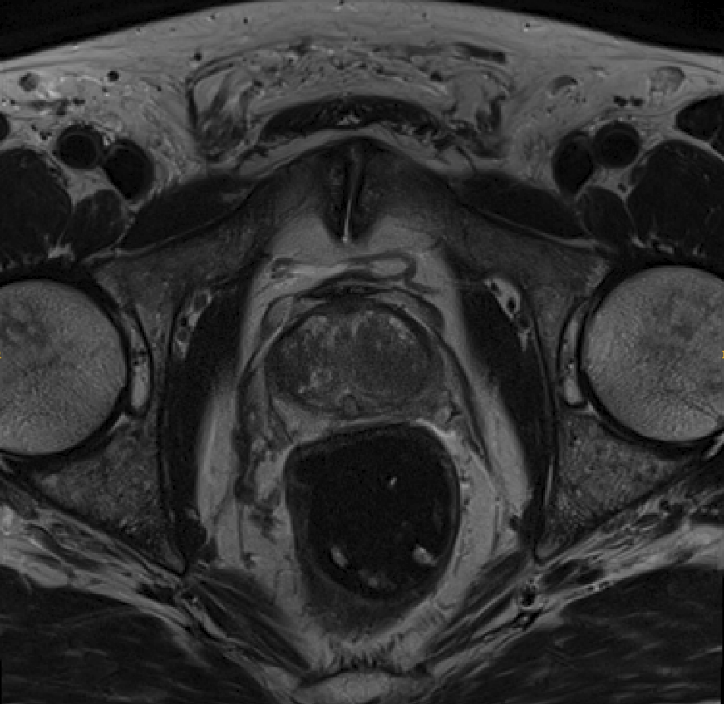
\includegraphics[totalheight=.15\textheight]{imgs/Preproc/Before.png}
    \hspace{10px}
    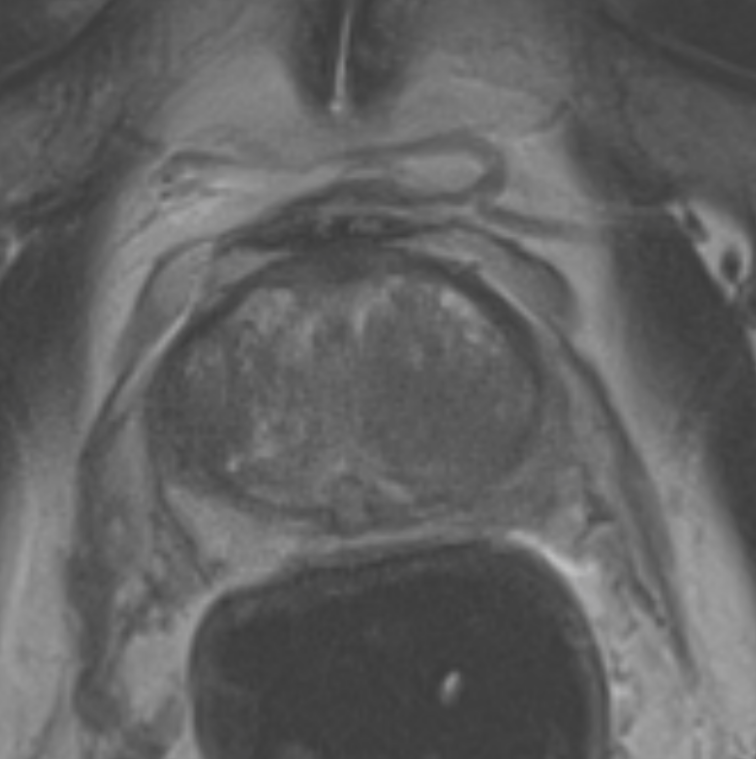
\includegraphics[totalheight=.15\textheight]{imgs/Preproc/After.png}
    \caption{In order to reduce the variability of the the MRI images from different magnets, they are pre-processed with bias correction, normalization, and cropped to a ROI.  In this example, the image on the left is the original data and the image on the right is the processed one. } \label{fig:roi}
\end{figure}

\begin{figure}[h]
    \centering
    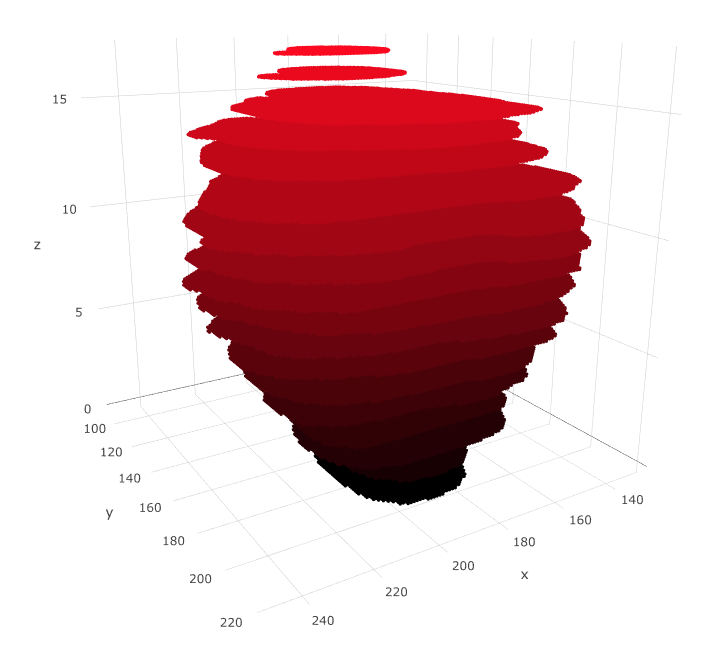
\includegraphics[totalheight=.15\textheight]{imgs/methodology/OF_1.png}
    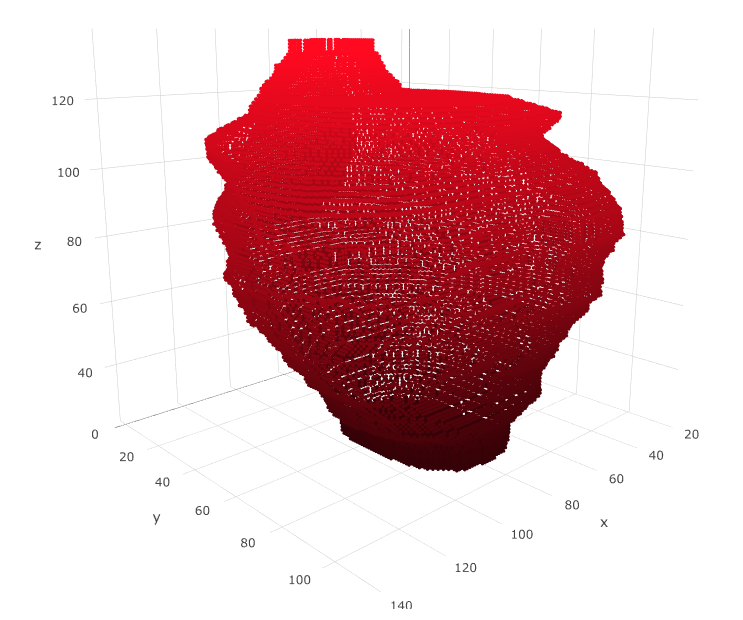
\includegraphics[totalheight=.15\textheight]{imgs/methodology/OF_2.png}
    \caption{Contours provided by experts are made on the original resolution of the MRI and interpolated using optical flow and linear interpolation to the higher resolution ROI. On the left: original contours with 17 slices. On the right: interpolated contours with 68 slices.}
    \label{fig:of1}
\end{figure}

\begin{figure*}[h]
    \centering
    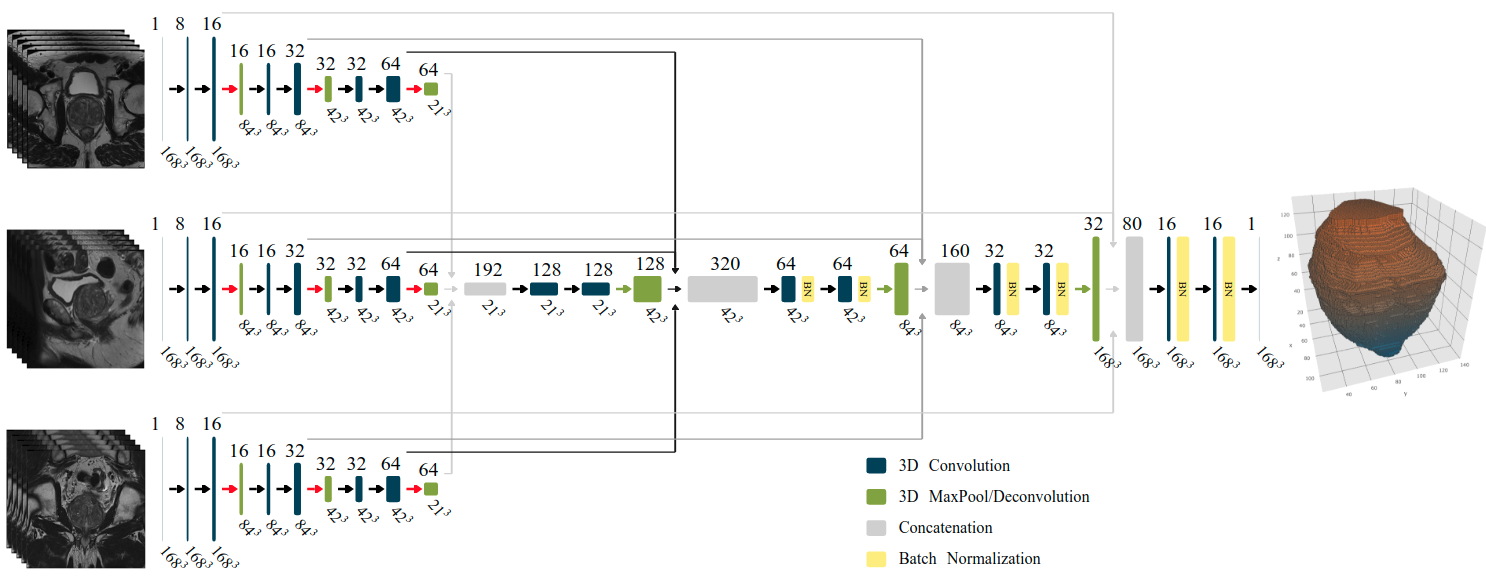
\includegraphics[totalheight=.275\textheight]{imgs/methodology/NN.png}
    \caption{Multistream 3D convolutional network architecture. The input of the network are $168^3$ volumes from the MRI planes: axial, sagittal, and coronal. }
    \label{fig:nn}
\end{figure*}

\begin{figure}[h]
    \centering
    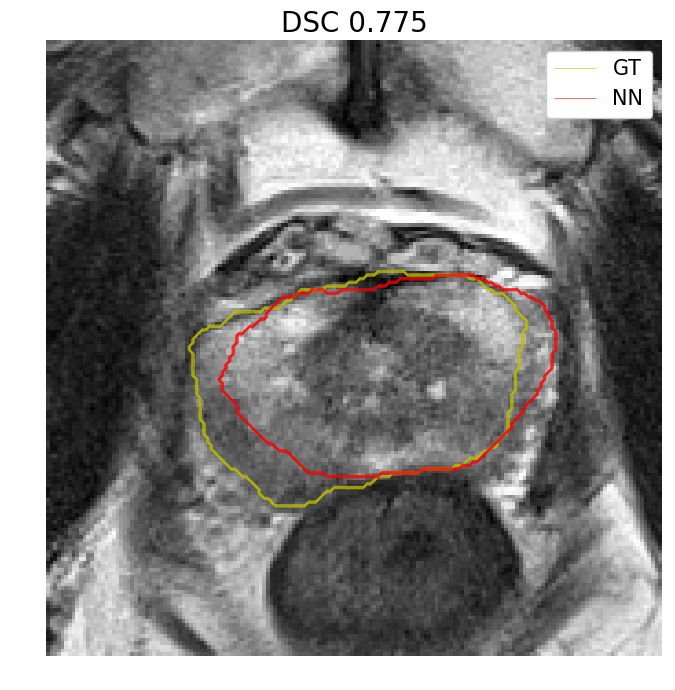
\includegraphics[totalheight=.2\textheight]{imgs/results/Prostate_Px_Challenge__P_yes_ROI_MIN_Case-0128.png}
    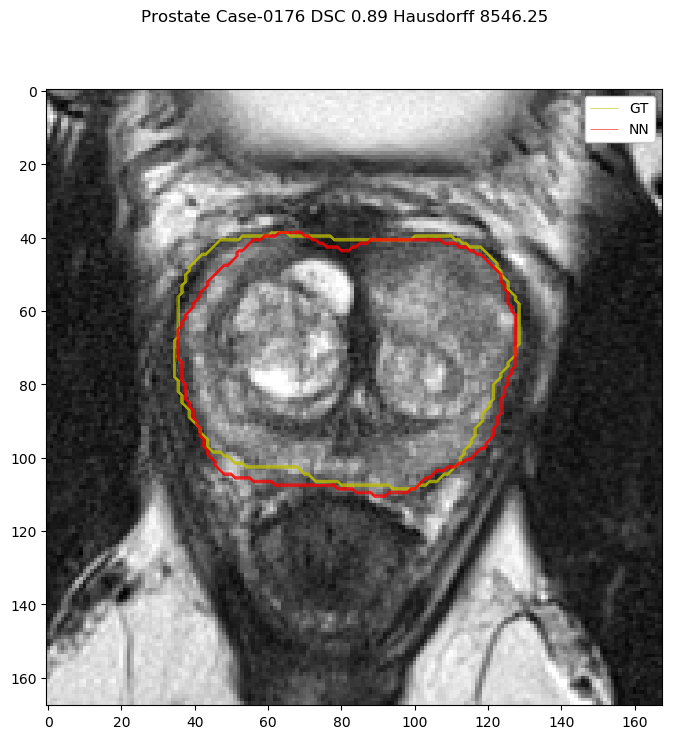
\includegraphics[totalheight=.2\textheight]{imgs/results/Prostate_Px_Challenge__P_yes_ROI_MEAN_Case-0176.png}
    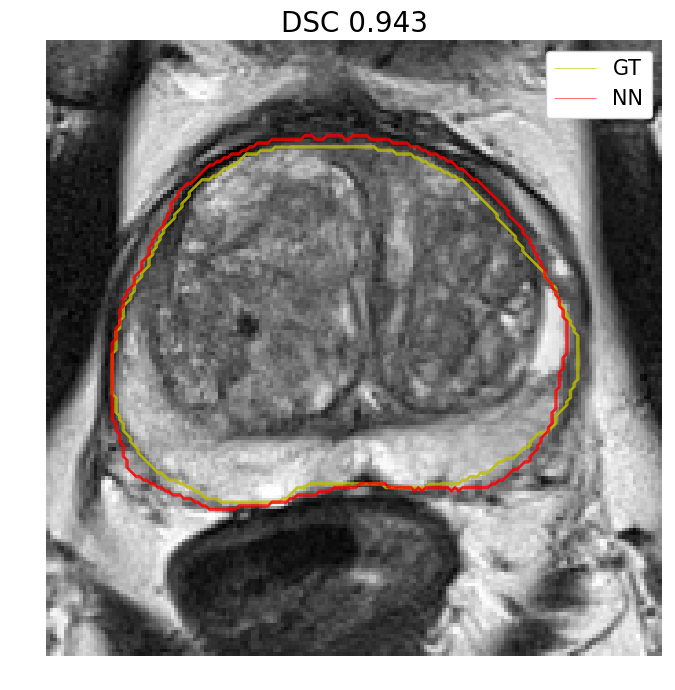
\includegraphics[totalheight=.2\textheight]{imgs/results/Prostate_Px_Challenge__P_yes_ROI_MAX_Case-0337.png}
    \vspace{10mm}
    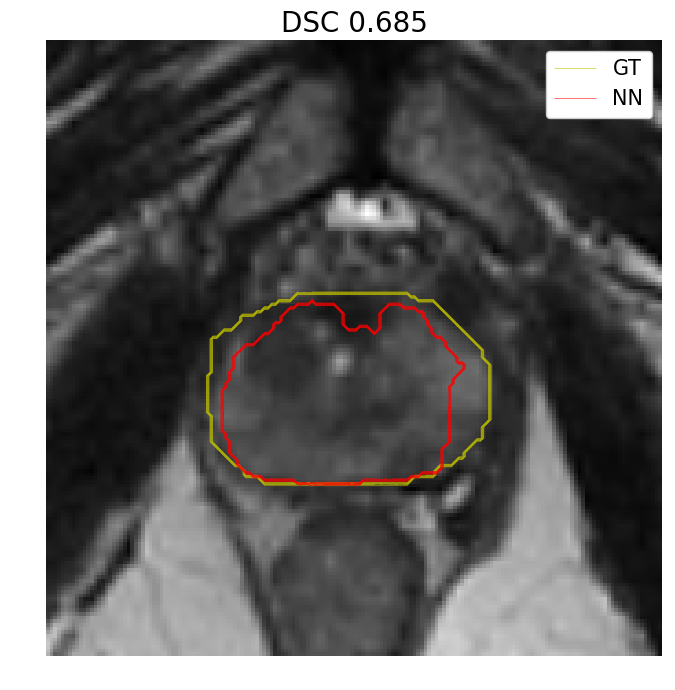
\includegraphics[totalheight=.2\textheight]{imgs/results/Prostate_GE__GE_yes_ROI_MIN_Case-0518.png}
    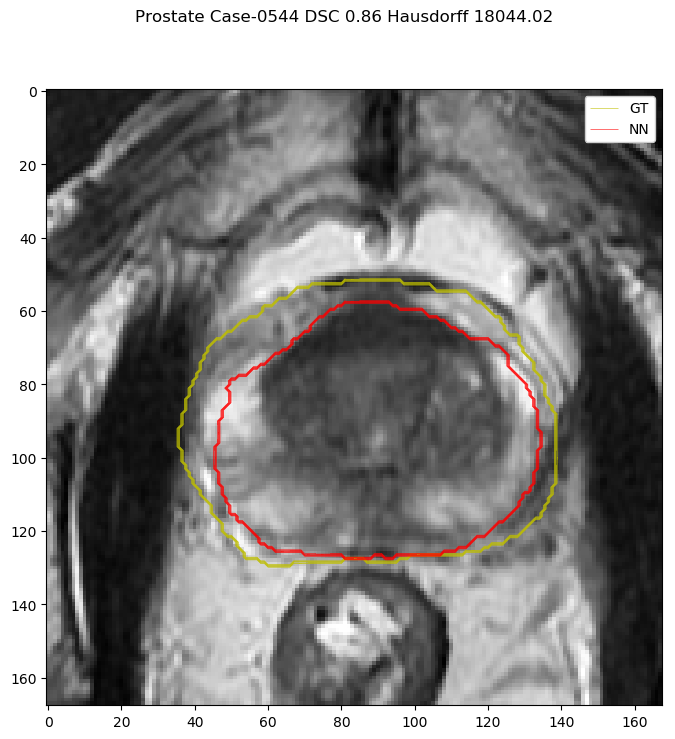
\includegraphics[totalheight=.2\textheight]{imgs/results/Prostate_GE__GE_yes_ROI_MEAN_Case-0544.png}
    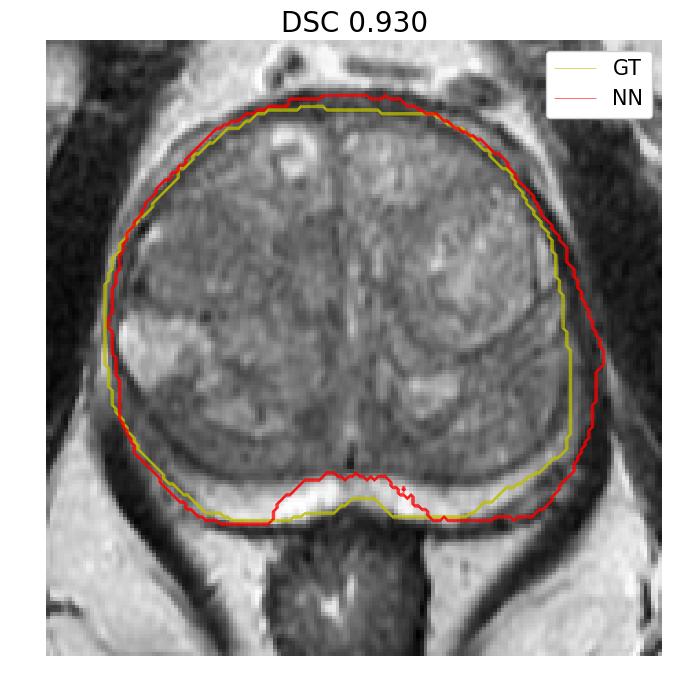
\includegraphics[totalheight=.2\textheight]{imgs/results/Prostate_GE__GE_yes_ROI_MAX_Case-0537.png}
    \caption{Segmentations of Siemens (up) and GE (down) MRI vendors respectively. }
    \label{fig:resseg}
\end{figure}

\begin{figure}[h]
    \centering
    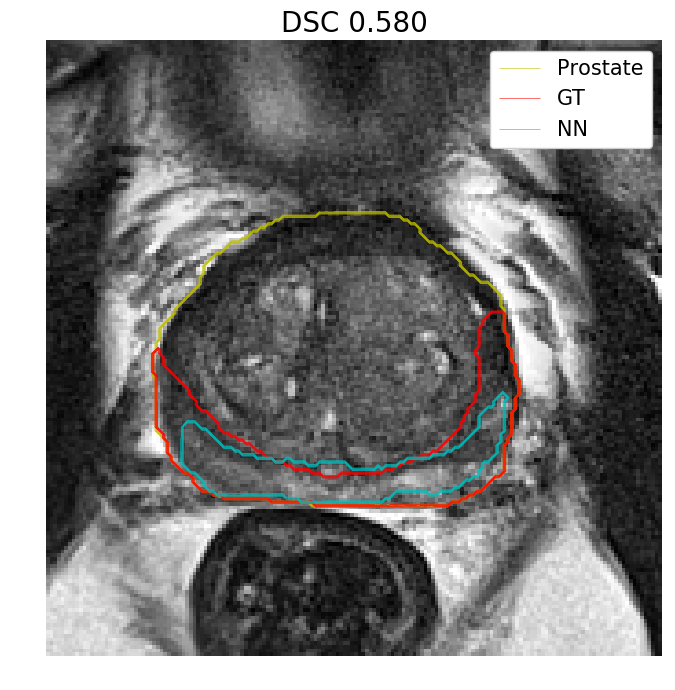
\includegraphics[totalheight=.2\textheight]{imgs/results/PZ_Px_Challenge__P_yes_ROI_MIN_Case-0300.png}
    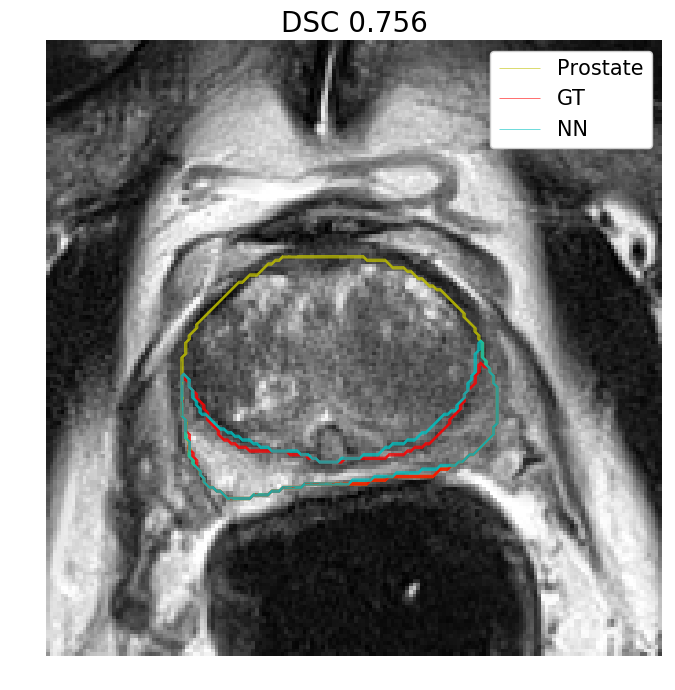
\includegraphics[totalheight=.2\textheight]{imgs/results/PZ_Px_Challenge__P_yes_ROI_MEAN_Case-0321.png}
    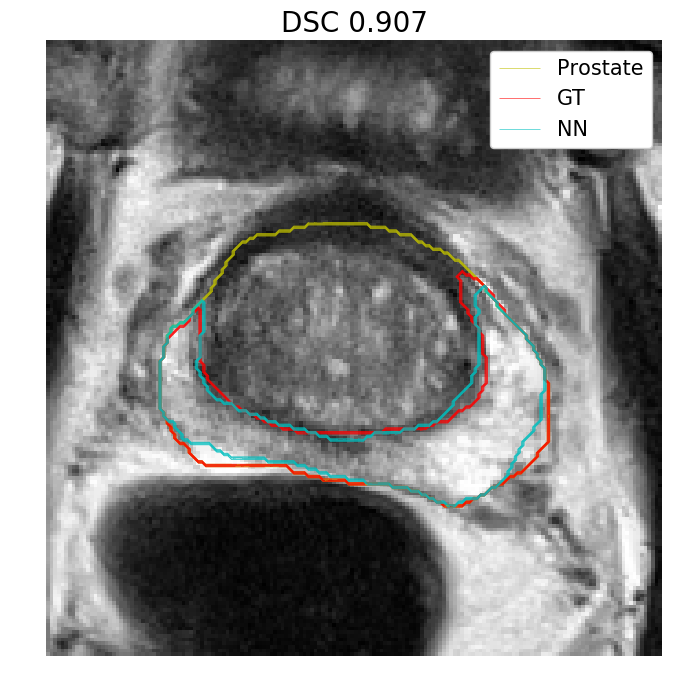
\includegraphics[totalheight=.2\textheight]{imgs/results/PZ_Px_Challenge__P_yes_ROI_MAX_Case-0028.png}
    \vspace{10mm}
    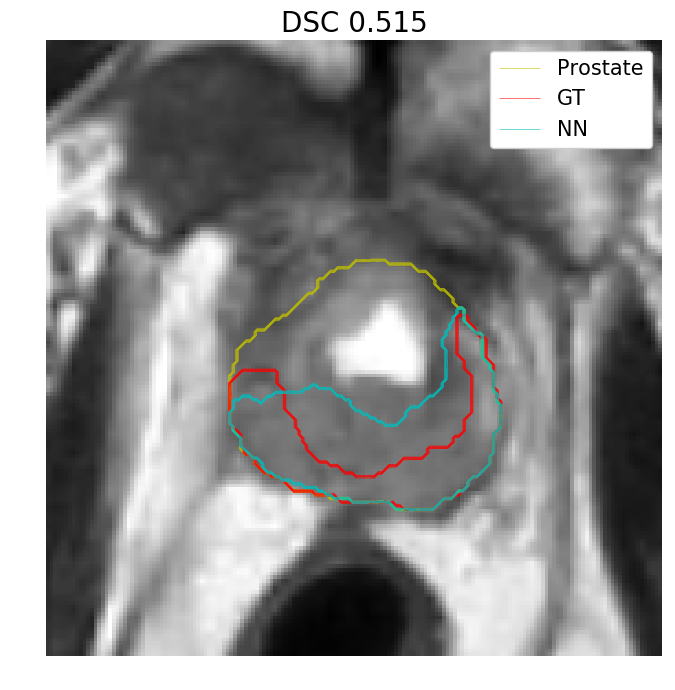
\includegraphics[totalheight=.2\textheight]{imgs/results/PZ_GE__GE_yes_ROI_MIN_Case-0383.png}
    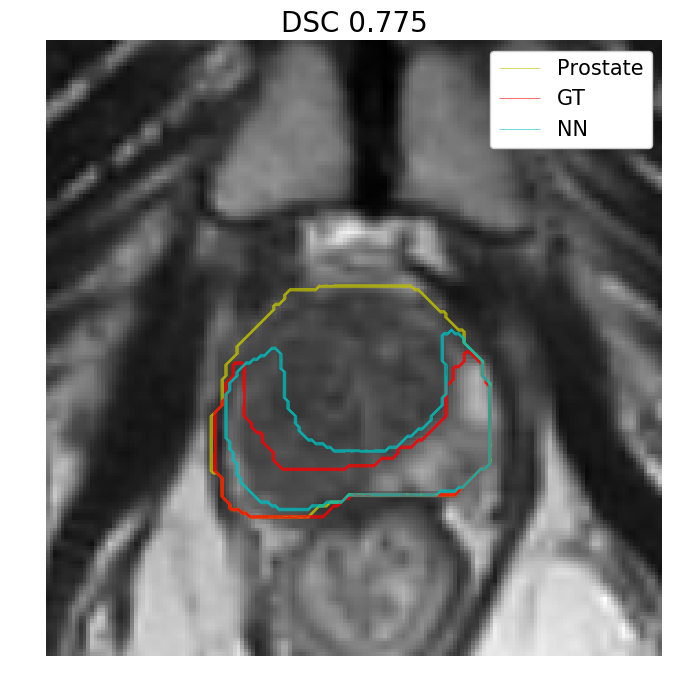
\includegraphics[totalheight=.2\textheight]{imgs/results/PZ_GE__GE_yes_ROI_MEAN_Case-0510.png}
    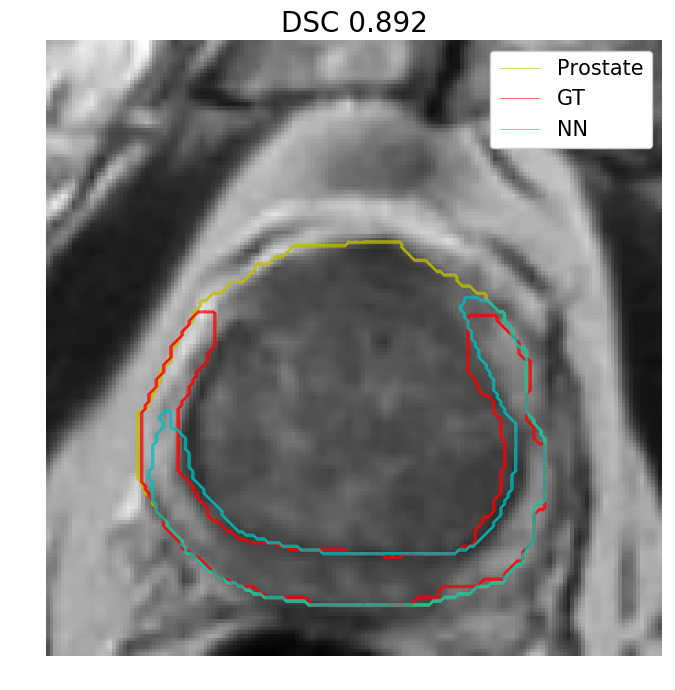
\includegraphics[totalheight=.2\textheight]{imgs/results/PZ_GE__GE_yes_ROI_MAX_Case-0441.png}
    \caption{Segmentations of Siemens (up) and GE (down) MRI vendors respectively. The obtained DSCs for these examples are 0.903 for the prostate and 0.737 for the peripheral zone.}
    \label{fig:ressegpz}
\end{figure}
